% !TEX TS-program = pdflatex
\documentclass[tikz,border=10pt]{standalone}
\usepackage{pgfplots}
\pgfplotsset{compat=1.18}
\begin{document}

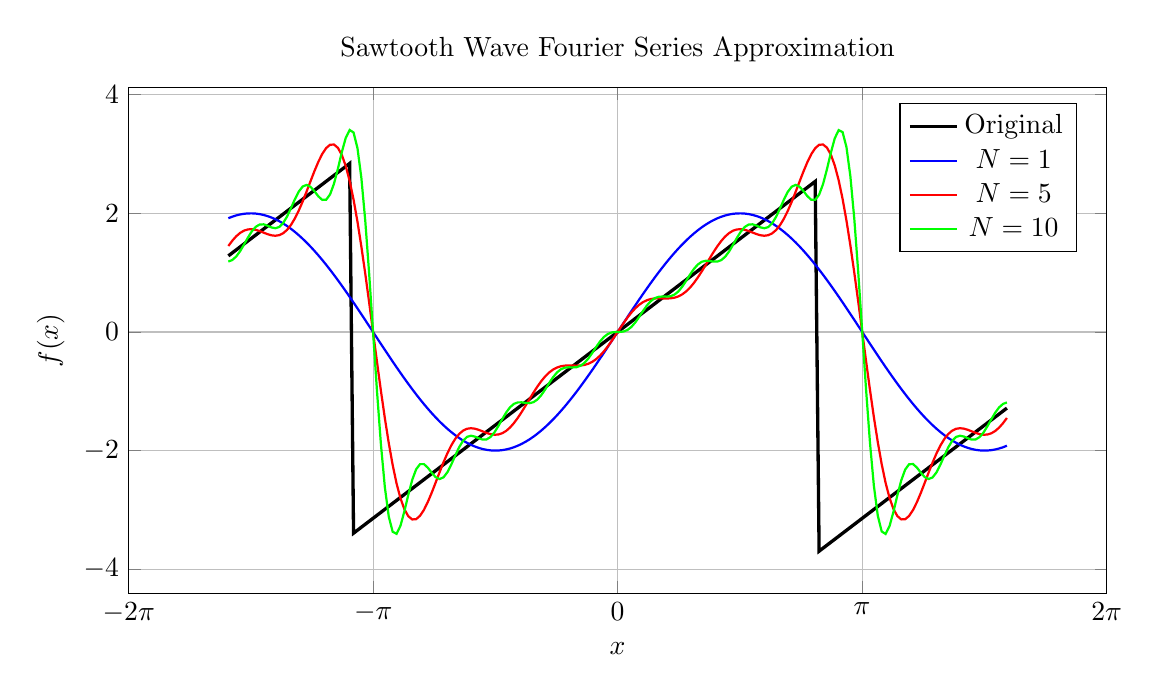
\begin{tikzpicture}
    \begin{axis}[
        width=14cm, height=8cm,
        xlabel={\(x\)},
        ylabel={\(f(x)\)},
        title={Sawtooth Wave Fourier Series Approximation},
        xmin=-6.28, xmax=6.28,
        grid=major,
        legend pos=north east,
        samples=200,
        xtick={-6.28, -3.14, 0, 3.14, 6.28},
        xticklabels={\(-2\pi\), \(-\pi\), \(0\), \(\pi\), \(2\pi\)},
        ]

        % Original sawtooth wave (periodic extension, shifted)
        \addplot[black, very thick] {mod(x + 3*pi, 2*pi) - pi};
        \addlegendentry{Original}

        \addplot[blue, thick] {2*sin(deg(x))};
        \addlegendentry{\(N=1\)}

        \addplot[red, thick] {2*(sin(deg(x)) - sin(deg(2*x))/2 + sin(deg(3*x))/3 - sin(deg(4*x))/4 + sin(deg(5*x))/5)};
        \addlegendentry{\(N=5\)}

        \addplot[green, thick] {2*(sin(deg(x)) - sin(deg(2*x))/2 + sin(deg(3*x))/3 - sin(deg(4*x))/4 + sin(deg(5*x))/5 - sin(deg(6*x))/6 + sin(deg(7*x))/7 - sin(deg(8*x))/8 + sin(deg(9*x))/9 - sin(deg(10*x))/10)};
        \addlegendentry{\(N=10\)}
    \end{axis}
\end{tikzpicture}

\end{document}